\documentclass{article}
\usepackage{tikz}
\usetikzlibrary{arrows.meta}

\begin{document}

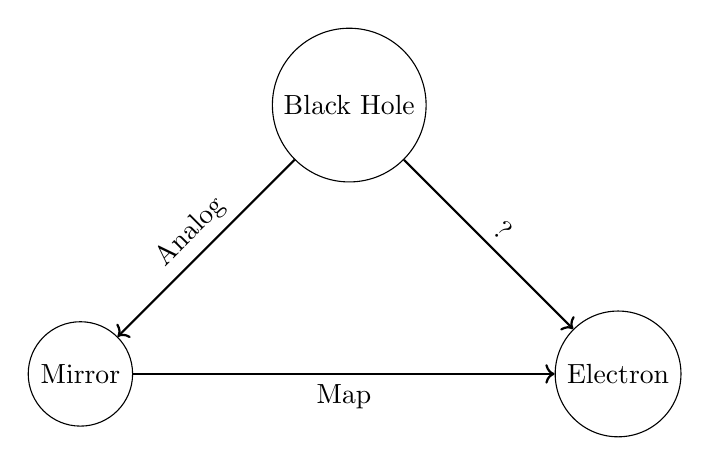
\begin{tikzpicture}[node distance=2cm]
    % Define nodes
    \node[circle, draw] (blackhole) {Black Hole};
    \node[circle, draw, below left of=blackhole, xshift=-2cm, yshift=-2cm] (mirror) {Mirror};
    \node[circle, draw, below right of=blackhole, xshift=2cm, yshift=-2cm] (electron) {Electron};

    % Draw arrows
    \draw[->, thick] (blackhole) -- node[midway, above, sloped] {Analog} (mirror);
    \draw[->, thick] (blackhole) -- node[midway, above, sloped] {?} (electron);
    \draw[->, thick] (mirror) -- node[midway, below, sloped] {Map} (electron);
\end{tikzpicture}

\end{document}